\documentclass[a4paper,10pt]{article}
\usepackage[utf8]{inputenc}
\usepackage[english]{babel}
\usepackage{indentfirst}
\usepackage{listings}
\usepackage{graphicx}
\usepackage{blindtext}
\usepackage{enumitem}
\usepackage{hyperref}
\usepackage[top=2.5cm,bottom=2.5cm,left=2.5cm,right=2.5cm]{geometry}
\pagestyle{headings}
\title{Ftp server in a datadiode}
\author{Rusu George, Boulif Ilias, Orinx Cédric}
\date{\today}

\begin{document}
\maketitle
\newpage
\tableofcontents
\newpage
\section{Concept of operations}
\subsection{Introduction to the problem}
Our client would want to prevent his research and development labs against industrial espionage and confidential information leaking. He wants to divide the company network in order to maintain the labs in an isolated environment. Thus, the critical data could not leave the company using the network. One problem related is assuring that all the operating systems are up to date. This could be achieved using a manual operation where an employee would manually update every node in the isolated network using a mass-storage device\footnote{A USB-key for instance.}. However, this is not the most optimized way and for sure it is not cost less and timeless for the company, without mentioning that there could be dependency problems. This method is prone to human errors and this could generate security vulnerabilities.

\subsection{Our solution}
In order to address this problem we are going to implement a data diode. In electronics as shown in Figure \ref{fig:diode}, a diode is a component which conduct the current in one direction. Thus the term of data diode is a set of components that only let the data to travel in an unidirectional way. An example of use case is illustrated in Figure \ref{fig:datadiode}, letting the data pass from a low risk VLAN\footnote{IEEE 802.1Q.} to a high risk VLAN but not the way around.
\begin{figure}
\centering
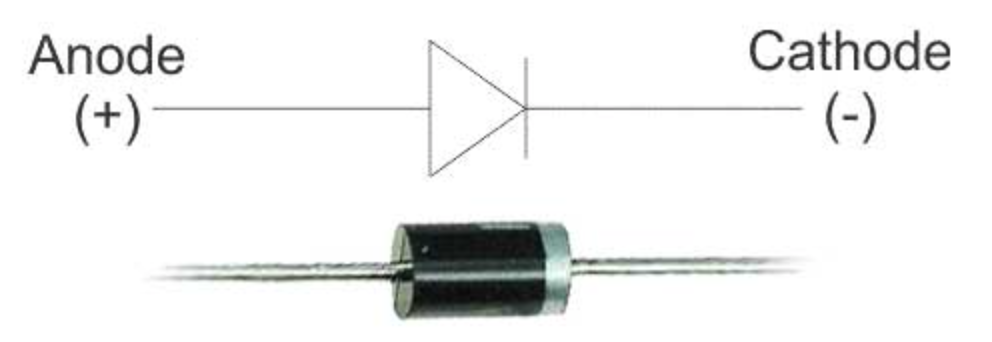
\includegraphics[scale=0.25]{images/diode.png}
\caption{A diode schema in electrionics.}
\label{fig:diode}
\end{figure}

\begin{figure}
\centering
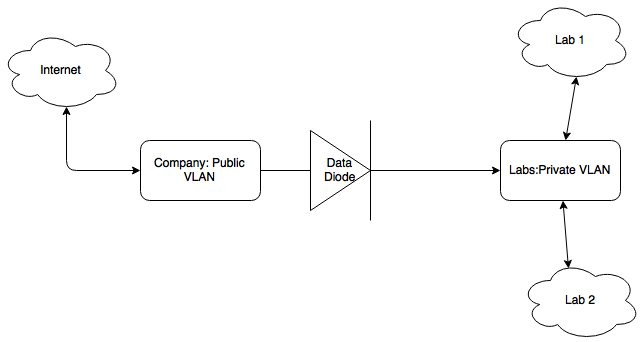
\includegraphics[scale=0.45]{images/dataDiode.png}
\caption{The schema of the usage of a data diode in a company network.}
\label{fig:datadiode}
\end{figure}

A data diode is made using one transmitter(Tx) and one receiver(Rx) both linked using only one fiber cable. Thus, when a digital data is send trough, every bit will be converted\footnote{Using a Digital to analog converter (DAC).} into an electrical pulse which will be convert in light pulse using a LED\footnote{Light Emitting Diode.}. Then, the output light will pass trough the fiber cable and as soon as the photons are reaching the receiver, they will be converted firstly into an electrical pulse by a photo diode and then in bits\footnote{Using an analog to digital converter (ADC).}. Since there is only one fiber, data can only travel in one way.

One major problem of this system is the network transport protocols(layer 4 in the OSI model) that applications are using. The most used transportation protocol nowadays is TCP. However, TCP is a bi-directional protocol which need the 3 way handshake in order to start a connection, thus there must be at least two fiber cables. In contradiction, UDP does not require a handshake process because it does not provide reliability, ordering, data integrity and does not set up a dedicated end-to-end connection automatically. Thus, UDP protocol does not necessary require a bi-directional data transfer. Therefore, the use of such a protocol is recommended when dealing with applications that are not sensitive to data loss or that implements an error checking system. Hence, the UDP protocol is used within the data diode.

It seems obvious now that the transport protocol used between the transmitter and the receiver of the data diode is UDP. However, this brings multiple problems. One of the problems is how to be able to use applications that requires TCP. Another problem could be the reliability of the digital data transfer in the data diode, how can we ensure that there will not be any data loss during the transfer. We will address to those questions further down in this document.\bigskip

Furthermore, system administrators would dispose of a file transmission mechanism from the low level to the high level in order to maintain all the computers up to date. This will be done using the FTP protocol and will be explained in the next section.

\subsection{Our System description}
The data diode concept is well orchestrated combination between hardware and software. The data diode is composed of two servers: a transmitter and a receiver. We could consider that the transmitter server is connected to the low security risk VLAN where a connection to the internet is made and where all the employees are connected. The receiver is connected to the high security risk VLAN where all the labs are connected and where critical informations is stored.

The transmission of the information will be from the low side to the high side and blocked the way around as shown in Figure \ref{fig:UDPDD}.

\begin{figure}
\centering
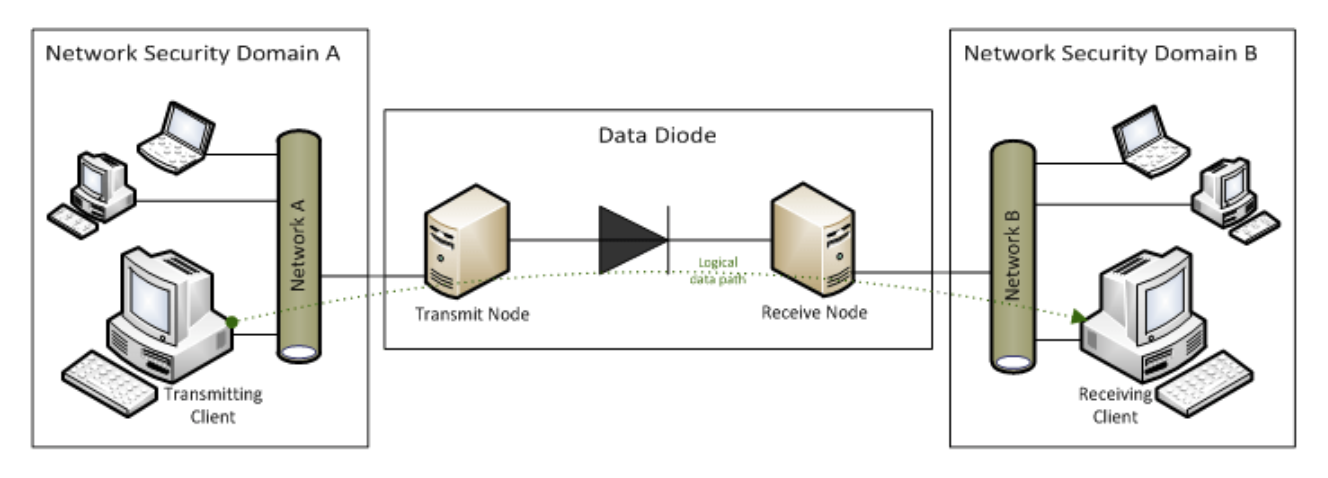
\includegraphics[scale=0.5]{images/logical-scheme-DD.png}
\caption{Data logical path within the data diode.}
\label{fig:UDPDD}
\end{figure}

\subsubsection{Hardware}
The following table presents the components used for the data diode implementation. We should mention that both transmitter and receiver possess two NICs\footnote{Network interface controller.}: one for the communication within the VLAN and one for the data diode.\bigskip
\begin{table}[!h]
\begin{tabular}{|p{3cm}|p{10.5cm}|}
	\hline
	\textbf{Components} & \textbf{Description}                 \\
	\hline
	Transmitter server  &  a physical machine or a virtual machine. The NIC for the data diode will be set in transmission mode only. \\
	\hline
	Receiver server  &  a physical machine or a virtual machine. Similar to the transmission, the nic will only be set in a receiver mode.\\
	\hline
	One fiber/UTP & This optical fiber allows communication between the low server the high server. It will probably be simulated using a UTP/RJ45 cable.\\
	\hline
	4 Fiber NIC/UTP NIC & Two for each server (transmission and receiver).  \\
	\hline
\end{tabular}
\caption{Components description}
\label{tab:component}
\end{table}
\subsubsection{Software}
We have chosen to use Linux as the main operating system for both transmission and receiver servers because of its reputation for safety and performance and also for its stability and efficiency in maintenance. The Linux distribution used in our project will be GNU Debian. 

The data diode will be easily administrated using a web interface running on an Apache server. The web site will be hosted on the transmission server. It will be described in more details further in this document.

Every configuration script used by the web interface will be a combination of Python language and Bash language.
\subsubsection{First overview on the project implementation}

Let's start by explaining which protocol shall be used in the data diode. Remember that our main goal is to create an isolated environment but also to facilitate the update process of the machines within the high security zone. As we mentioned earlier, we are going to use the FTP\footnote{File transfer protocol.} protocol. There are some alternatives to FTP such as BlindFTP, SFTP, etc. However FTP and SFTP are using TCP as their transportation layer protocol. Thus, we are going to use between the transmitter and the receiver the BlindFTP which is use UDP instead.

BlindFTP is a simple Python script which was especially created for the communication between the two servers over an unidirectional network. It is simply a tool for transferring files from one side to the other. Despite the fact that use UDP, there is no acknowledgement of received packets but this is compensated by a redundancy of the data. An other advantage is the language used, as it is written in Python the result code is relatively simple and very portable to Windows or MacOS.

It is now time to have a look to our entire system, let's have a look in Figure \ref{fig:sysschem}.\bigskip

\begin{figure}
\centering
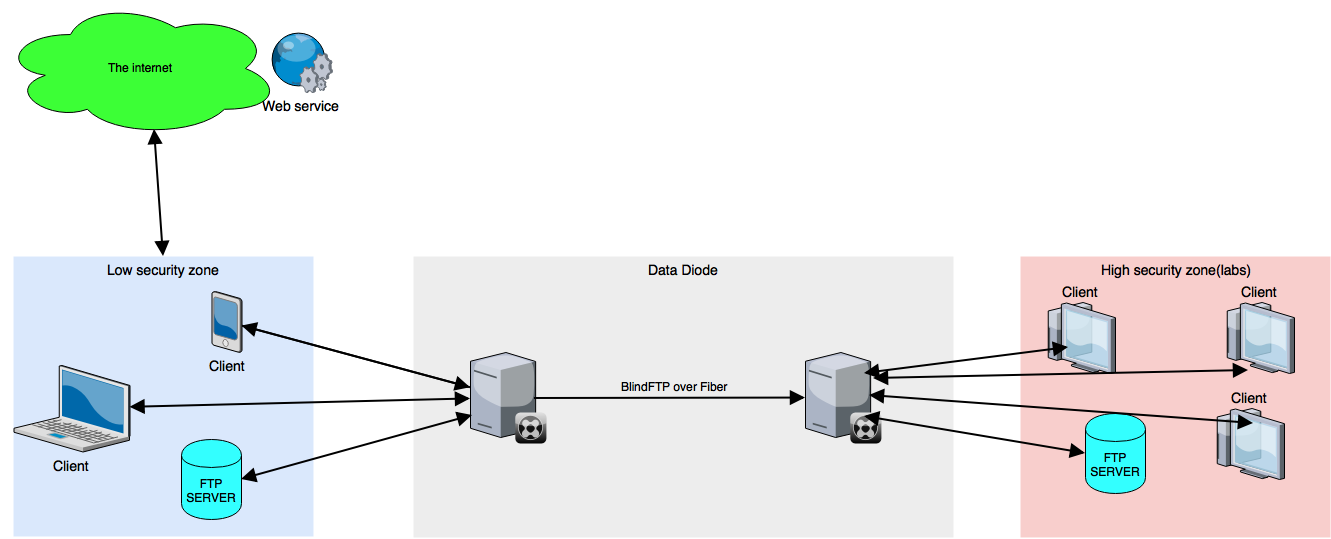
\includegraphics[scale=0.35]{images/systemschema.png}
\caption{Entire system.}
\label{fig:sysschem}
\end{figure}

Using BlindFTP allows us to ignore if the application is using TCP or UDP, the only thing we need is to make sure that the data arrive to the transmitter. We should note that between the transmitter and the other peers a TCP connection can be used to communicate. And this is the same for the receiver, after the data goes out from the network diode the transportation protocol could be TCP with other peers. In this way, we are not dealing any more with the problem of application transportation layer. 

\subsection{Users} 
In general every employee of a company has a unique ID, a grade, a job title, etc. The company owner or the manager in charge with the security could choose which grade or which person can have access to the administration web interface, of course this exclude the systems administrators.  Thus to make our explanation simple, let's suppose that there will be two types of users in our system : the \textit{administrators} and the all the other\textit{users}.

A \textit{user} is simply an employee of the company. Every employee have limited access into the company's files according to their job title or to the specific rule defined by their supervisor.

An \textit{administrator} is a user in charge of operating and maintaining the data diode. It is the only authorized person to interact with the data diode and this is mandatory. Because he will have to know how the data diode is working, should know how to interact with it using the web interface but mostly he should be able to reconfigure it or restore it as quickly as possible in case of a security breach or a system failure. However, an administrator could not have access to some strict secret files of the company but only to the used IT mechanism.

Every user information is managed and stored by the company in their own databases.
\subsection{User Interface}\label{UI}

As we mentioned earlier, the administration of our data diode will happen through a web interface. This web interface will be hosted on the transmitter and will allows to transmit files or update packages from the lower network to the higher network.

Here is an overview on our web interface:

SCREEN PAGE PRINCIPALE

DIRE PAR EXEMPLE QUE LES USER ONT UN ACCES JUSTE POUR FTP ET QUE LES ADMIN ON TUN ACCES JUSTE POUR LES MISE A JOUR, PAR EXEMPLE ON PEUT AUSSI DIRE QUE POUR UN FTP ON A UNE FORME AVEC UPLOAD FILE ET PUIS UN SEND FILE , POUR LES ADMIN ON AURAI UN BOUTTON AVEC RECHERCHE DE MISE A JOUR, PAR LA SUITE ON AURAIT TELECHARGER LES MISE A JOURE SELECTIONNéE ET LES ENVOYé DE L'AUTRE COTE. 

ON POURRAI AJOUTER POUR LE COTE ADMIN, ET POUR LES MANAGER, UN ESPECE D'HISTORIQUE AVEC QUI A FAIT QUOI, QUI A UPLOADE QUOI, QUI A MIS A JOUR, -> FONCTIONNALITé DE TRACAGE , ON POURRAI AUSSI AVOIR UN HISTORIQUE DE TOUT LES MISE A JOUR DEJA FAIT, PAREIL POUR LES FICHIER DE L'AUTRE COTE DEJA ENVOYE ( ICI COMMENT SAVOIR SI LE FICHIER EST ENCORE LA OU PAS? )


AU NIVEAU DE L'INTERFACE, J'IMAGINE CA TRES SIMPLEMENT AVEC UNE PAGE, AVEC AU DEBUT UN LOGIN AVEC MOT DE PASSE (LIE A CE QUE J'AI DIT DANS LA PARTIE USER) APRES EN FONCTION DU JOB TITLE (SOIT UN CHERCHEUR SOIT UN ADMIN) ON VA AVOIR LES PAGES RESPECTIVENT QUI S'AFFICHE, 

-USER -TRANSFERT DE FICHIER
-ADMIN - MISE A JOUR

POUR USER, JE VOIS CA AVEC UNE FORME OU ON PEUT UPLOADER UN FICHIER, AJOUTER UNE DESCRIPTION ET L'ENVOYER, DE L'AUTRE COTE COMME UN COMMIT SUR GITHUB

COTE ADMIN J'IMAGINE AVOIR UN PANEL (TABLEAU) DANS LEQUEL ON VA LISTER TOUT LES MISE A JOUR DISPONIBLE DEPUIS UNE CERTAINE DATE( DERNIERE MISE A JOUR) ET ENSUITE POUVOIR EN TANT QU'ADMIN FAIRE UNE SELECTION DES PACKAGE QU'ON AIMERAI TRANSMETTRE. DU COUP ON PEUT SELECTION ET TRANSFERER DE L'AUTRE COTE.

EN PLUS DE CA FAUT DIRE QUE NOTRE FTP SERVEUR EST DIVISER EN PLUSIEUR BRANCHE, GENRE BRANCHE ADMIN BRANCHE CHERCHEUR, ETC... DU COUP L'UTILISATEUR AVEC SON COMPTE N'A ACCES QUE A SON PROPRE ESPACE. -> PEUT-ETRE HORS DU PROJET MAIS ON PEUT L'ENONCER ET DIRE QUE CA POURRAIT ETRE TRES FACILEMENT MIS EN OEUVRE.

ENSUITE POUR CHAQUE PARTIE ESSAYER DETAILLER BETEMENT QUEL BOUTTON FAIT QUOI, COMMENT SE LOGER EN ETAPES AVEC DES NUMERO ET TOUS CA DANS LA PROCHAINE SECTION COMMENT.


[idee : site web sur le transmitter, login+ mot de passe , avoir une certainte tracabilité, pouvoir umploader une fichier depuis le site et juste l'envoyer de l'autre cote. ]\\


\subsection{General usage}
The interface will be used each time by the users from the secured network
in order to transfer a file through the data diode. By using the interface,
users can transfer the files they need by simply dragging and dropping them to
the dedicated transfer folder which is forwarded to the secure network.

There is the s
\begin{enumerate}
\item[-] 
\end{enumerate}
easy to use. In ordre to use the interface, the first step is to log on with his
user name and password.  Once we are connected, (if we are a user??)
we are on a page that allows the file transfer from the transmitter(lower network)
to the receiver(high network), simply by a mechanism of drag and drop(or upload?).
(if we are admin??)


\begin{thebibliography}{9}


\bibitem{data-diode-work}
DEEP SECURE,
\textit{How	Does a Data Diode Work?}
Discussion Paper, February 2017.

\bibitem{data-diode-SANS-Institute}
SANS Institute InfoSec Reading Room,
\textit{Tactical Data Diodes in Industrial Automation and Control Systems}, January 2015.

\bibitem{data-diode-transport}
CS Risk Management and Compliance Ltd,
\textit{Data Diode vs Firewall Feasibility}, September 2016. [Online]. Available: \url{https://csriskmanagement.co.uk/data-diode-vs-firewall-feasibility/} [Accessed: 30- Oct- 2017]
\bibitem{data-diode-transport}

BlindFTP,
\textit{Blind ftp protocol}[Online]. Available: \url{https://www.decalage.info/fr/python/blindftp} [Accessed: 30- Oct- 2017]

\end{thebibliography}
\end{document}